\documentclass[10pt]{scrartcl}

\usepackage[utf8]{inputenc}
\usepackage{tabularx}
\usepackage{longtable}
\usepackage[ngerman]{babel}
\usepackage[automark]{scrpage2}
\usepackage{amsmath,amssymb,amstext}
%\usepackage{mathtools}
\usepackage[]{color}
\usepackage[]{enumerate}
\usepackage{graphicx}
\usepackage{lastpage}
\usepackage[perpage,para,symbol*]{footmisc}
\usepackage{listings} 

\usepackage[numbers,square]{natbib}
\usepackage{color}
\usepackage{colortbl}
\usepackage[absolute]{textpos}
\usepackage{float}
\usepackage[colorinlistoftodos,textsize=small,textwidth=2cm,shadow,bordercolor=black,backgroundcolor={red!100!green!33},linecolor=black]{todonotes}
\usepackage[pdfborder={0 0 0},colorlinks=false]{hyperref}
\usepackage[all]{hypcap}

\lstset{numbers=left, numberstyle=\tiny, numbersep=5pt, breaklines=true, showstringspaces=false} 
\restylefloat{figure}

%changehere
\def\titletext{Praktikum 1 : Stellen/Transitionsnetze}
\def\titletextshort{Praktikum 1}
\author{André Harms, Oliver Steenbuck}

\title{\titletext}

%changehere Datum der Übung
\date{04.04.2012}

\pagestyle{scrheadings}
%changehere
\ihead{TH1, Padberg}
\ifoot{Generiert am:\\ \today}

\cfoot{Oliver Steenbuck, André Harms}


\ohead[]{\titletextshort}
\ofoot[]{{\thepage} / \pageref{LastPage}}

\setlength{\parindent}{0.0in}
\setlength{\parskip}{0.1in}

\begin{document}
\maketitle

\setcounter{tocdepth}{3}
\tableofcontents

%	\listoftables                                 												% 
	\listoffigures  
	\lstlistoflistings	

\section{Modellierung}
	Abbildung \ref{img:aufg1} zeigt das hier gewählte Modell für das in der Aufgabe beschriebene Zusammenspiel von Sender un Empfänger. Im Folgenden auf die in der Modellierung getroffenen Entscheidungen und ihre Alternativen eingegangen und für einige ausgewählte Alternativen diese an den Modellen der Teilaufgaben Fünf und Sechs gezeigt.
	  
	\begin{figure}[H]		
        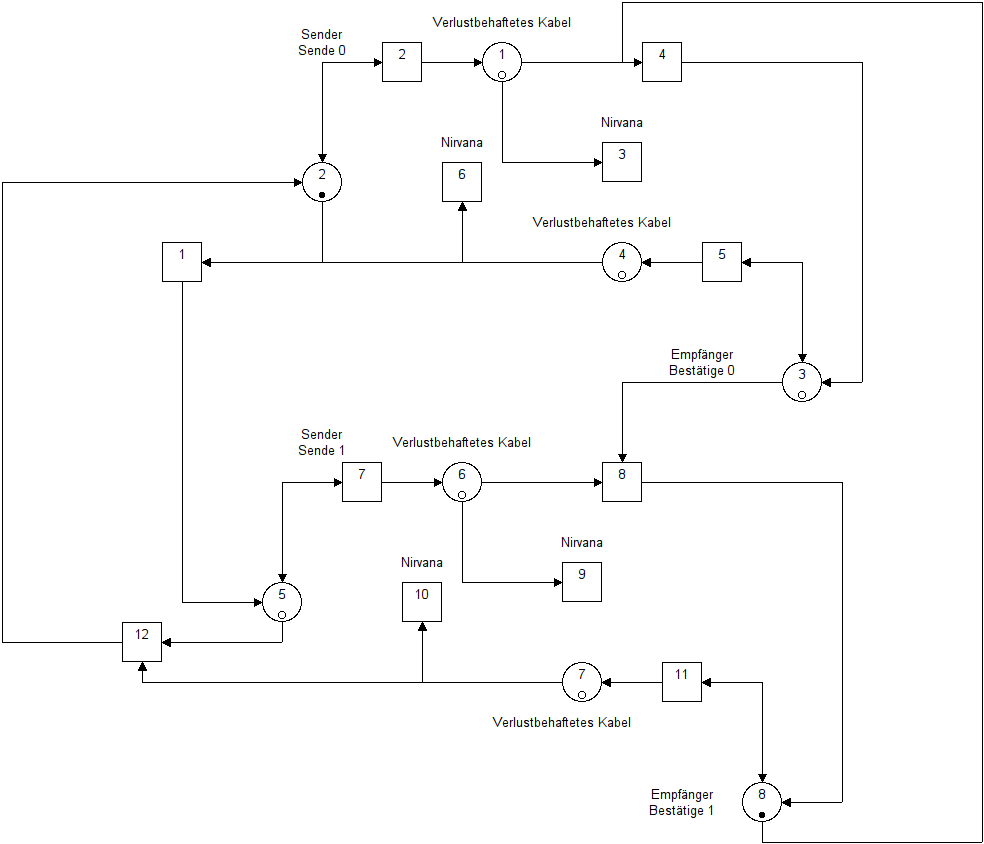
\includegraphics[scale=0.5]{praktikum1-aufgabe1.png}
        \caption{Teilaufgabe 1: Petri Netz} 
        \label{img:aufg1}
	\end{figure}
	
\subsection{Modelannahmen}

Es wird hier\footnote{Teilaufgabe Eins} nur das Kabel modelliert und keine Details des Empfängers. In Abbildung \ref{img:aufg1} ist dies Berispielhaft in den Verbindungen der Plätze \verb!2! und \verb!3! zu erkennen. Die als \verb!Nirvana! bezeichnete Transistion \verb!3! ist die einzige in der Nachrichten verloren gehen können und repräsentiert somit sowohl Verluste auf dem Kapel als auch beim Empfänger. Die Transisiton \verb!4! die den Übergang einer Nachricht vom Kabel in den Empfänger konsumiert aus dem Platz \verb!8! die Bestätigungsnachricht für das andere Bit die nun nicht mehr gesendet werden kann.
Die Kompelxität liegt hier in der Modellierung des verlustbehafteten Kabels. Alternativ wäre eine Modellierung denkbar bei der auf Empfängerseite noch weitere Details ausgearbeietet werden, siehe auch Abbildung \ref{img:aufg5}.

In der hier gewählten Modellierung ist keine globale Taktung vorhanden. Dieser Weg wurde gewählt um die Modellierung nicht übermäßig komplex werden zu lassen. Es lassen sich so mit dem petri-Netz allerdings Effekte simulieren die in der Realität schwer vorstellbar sind. Beispielhaft sei das 1000 malige Senden der Bestätigung in der Zeit in der nur eine Nachricht gesendet wurde genannt.   
Alternativ könnte durch das Einteilen des Netzes in verschiedene Aktoren die jeweils eine Aktion ausführen können wenn sie ein globales Token besitzen eine Taktung hergestellt werden die die Simulation näher and die Realität führt. 

In Teilaufgabe Eins werden die verlorengegangenen Nachrichten nicht gezählt. Wenn ein Simulationstool gewählt wird das nicht vom Anwender gesteuert wird (beispielsweise \verb!Snoopy!) sollten zur statistischen Auswertung Plätze zum Sammeln und Zählen der verlorengegangenen Nachrichten geschafen werden, ein solches Zählen ist beispielhaft in Abbildung \ref{img:aufg5} Platz 6. 

\subsection{Bedeutung von Token}
Ein Token in unserem Graphen repräsentiert entweder eine Nachricht oder eine potentielle Nachricht.
Genauer ausgeführt repräsentiert ein Token auf folgenden Plätzen Nachrichten:
\begin{itemize}
	\item 1
	\item 4
	\item 6
	\item 7
\end{itemize}
Auf anderen Plätzen repräsentiert ein Token das Potential das von hier aus, in der aktuellen Konfiguration eine Nachricht erzeugt werden kann. 
In den anderen Teilaufgaben (5 und 6) ist die Aufteilung ähnlich, auf em Kabel repräsentiert ein Token eine Nachricht an den anderen stellen das Potential eine Nachricht versenden zu können. Wobei teilweise ein Token nur einen Bruchteil einer Nachricht repräsentiert. Beispielsweise  in Teilaufgabe 6 (Abbildung \ref{img:aufg6}) Platz 9, hier ist jeder Token $\frac{1}{20}$ einer Nachricht.	
	
	
\section{Korrektheit}
Um die Korrektheit des in Abbildung \ref{img:aufg1} gezeigten Netzes zu beweisen haben wir den Erreichbarkeitsgraphen (siehe: Listing \ref{lst:eGraph}) des Netzes darauf untersucht, dass er nur legale Konfigurationen enthält.
Jede legale Konfiguration erfüllt folgende Bedingungen:
\begin{itemize}
	\item Genau ein Token auf 2 oder 5
	\item Genau ein Token auf 3 oder 8
\end{itemize}

Die Prüfung der in Listing \ref{lst:eGraph} enthaltenen Nodes auf die Erfüllung dieser Bedingungen zeigt, daß das Netz ausgehend von der in Abbildung \ref{img:aufg1} gezeigten Startkonfiguration nur legale Zustände erreichen kann.

\lstinputlisting[label=lst:eGraph, frame=single, caption={Nodes im Erreichbarkeitsgraphen}]{ErreichbarkeitsGraphAufg1.txt}

\subsection{Nachrichtenverlust}
Im hier gewählten Modellierungtool ist die Anzahl an verlorengegangenen Nachrichten abhängig von Benutzereingaben. Gegeben ein Tool das alle Ausgänge gleichwertig behandelt würden wir mit einem Nachrichtenverlust von ca. 50 Prozent rechnen.

\section{Petri Netze}
	Im foglenden sind die Netze für Teilaufgabe 5 in Abbildung \ref{img:aufg5} und Teilaufgabe 6 in Abbildung \ref{img:aufg6} gezeigt.

	\begin{figure}[H]	
        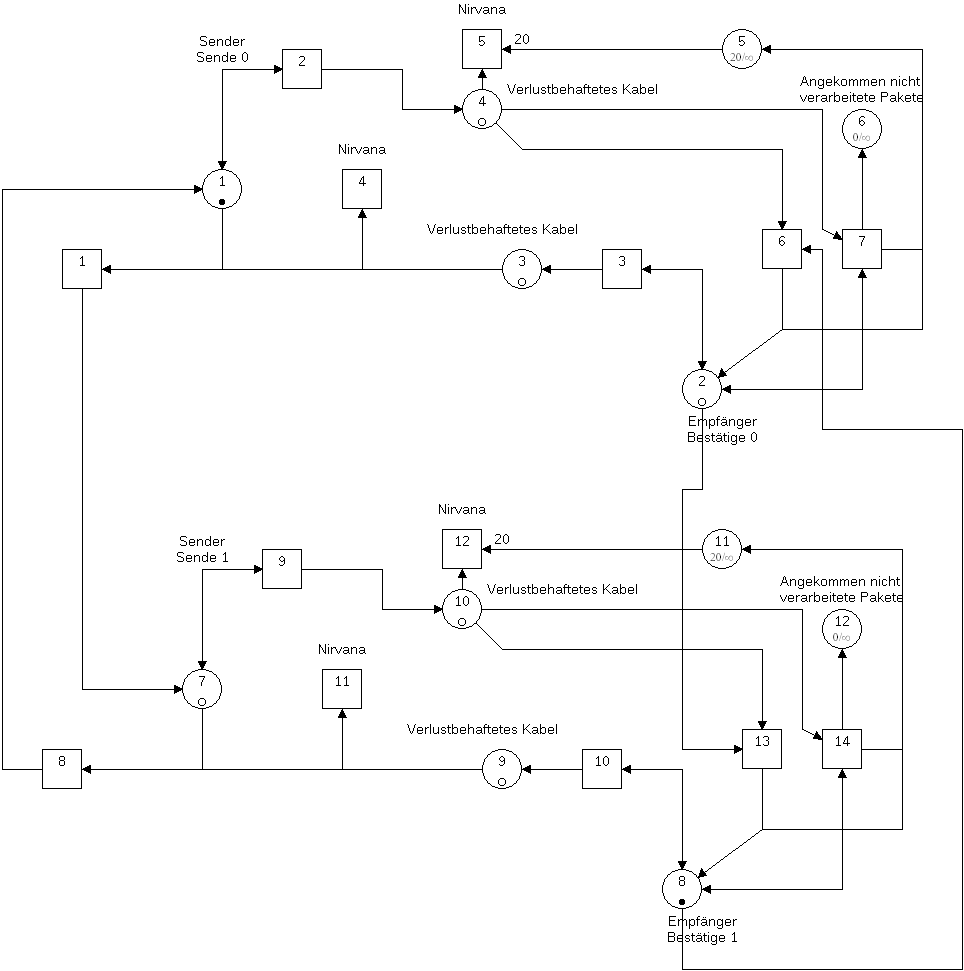
\includegraphics[width=\textwidth]{praktikum1-aufgabe5.png}
        \caption{Teilaufgabe 5: Petri Netz}  
        \label{img:aufg5}
	\end{figure}


	\begin{figure}[H]
        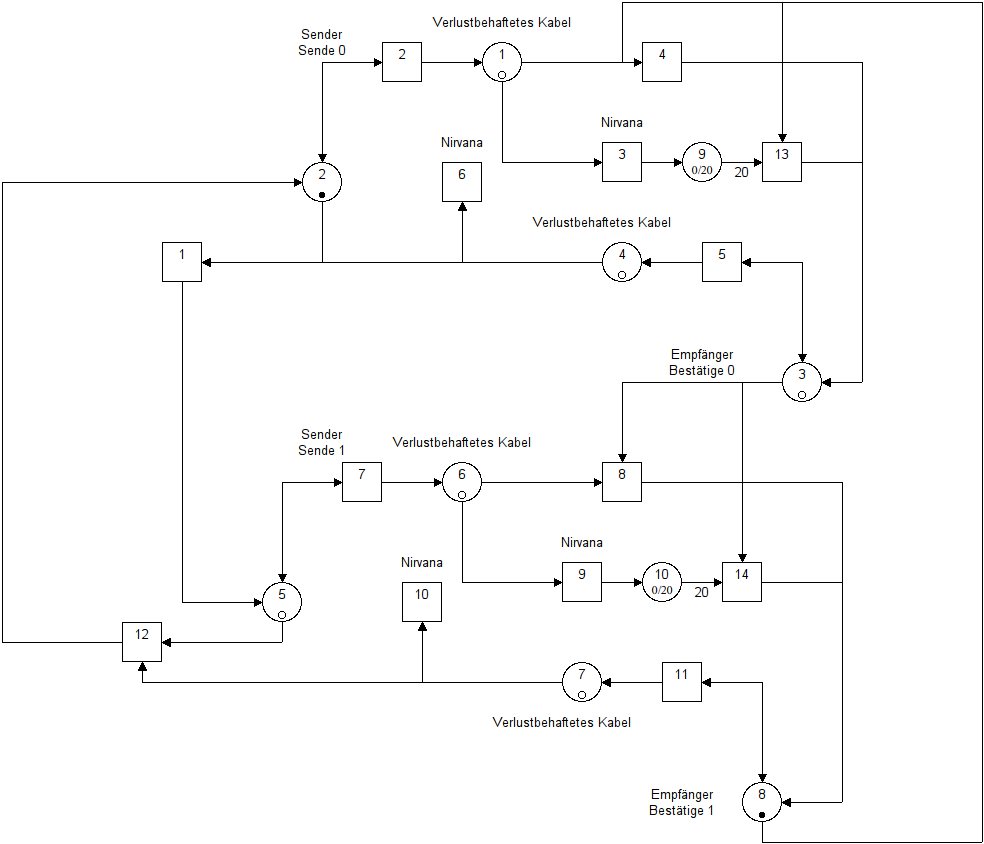
\includegraphics[width=\textwidth]{praktikum1-aufgabe6.png}
        \caption{Teilaufgabe 6: Petri Netz}   
		\label{img:aufg6}   
	\end{figure}

\end{document}

